%%%%%%%%%%%%%%%%%%%%%%%%%%%%%%%%%%%%%%%%%%%%%%%%%%%%%%%%%%%%%%%%%%%%%%
% This layout was adapted from one found at latextemplates.com which
% was adapted from another.
%
% License: CC BY-NC-SA 3.0
% (http://creativecommons.org/licenses/by-nc-sa/3.0/)
%
% Original header:
%
% This is a LaTeX version of the sample laboratory report from
% Virginia Tech's copyrighted 08-09 CHEM 1045/1046 lab manual.
% Reproduction of this one appendix section for academic purposes
% should fall under fair use.
%
%%%%%%%%%%%%%%%%%%%%%%%%%%%%%%%%%%%%%%%%%%%%%%%%%%%%%%%%%%%%%%%%%%%%%%

\documentclass{article}

\usepackage{graphicx} % Lets us use images
%\usepackage[acronym]{glossaries} % Lets us use acronyms
\usepackage{siunitx} % SI units in math mode

\author{}
\title{ELEC-313 \\ Lab 1: Amplifier Models \\ }
\date{\today}

% This loads the acronym definitions and creates a glossary.
% \makeglossaries is required (I think), even though we don't print
% out a separate glossary page.  The first time an acronym is used,
% LaTeX writes the whole word (defining the acronym), and after that
% it prints only the acronym.  There is an example of their use in the
% caption of the table in the Results section.
%\loadglsentries{acronyms} % Actually loads 'acronyms.tex'
%\makeglossaries

\begin{document}

\maketitle % Inserts title, author, and date from above

 \begin{center}
   \begin{tabular}{lr}
     Date Performed: & September 11, 2013 \\
     Partners: & Charles Pittman \\
               & Stephen Wilson \\
  \end{tabular}
\end{center}

\pagebreak

% Removes indentation from paragraphs: \setlength\parindent{0pt}

% Number the enumerate environment (unordered lists) by letter:
\renewcommand{\labelenumi}{\alph{enumi}.}

% And now we start our actual text.  Note that each chunk is
% designated by the \section{} tag.
\section{Objective}
% \label{} is used when you want to refer to something later.  It's
% simply an identifier for whatever container it's in.  See
% Conclusions section for an example of \ref{}.
\label{sec:objective}

The objective is to verify the equivalence of four circuits used to
model an amplifier, shown in Figure~\ref{fig:amp_models}.

\section{Schematics}
\label{sec:schematics}

% The asterisk after section inhibits the numbering of the section.
\subsection*{Circuit Tested}
\label{sec:ckt_tested}

% Insert a picture:
\begin{figure}[hbtp]
  \centering
    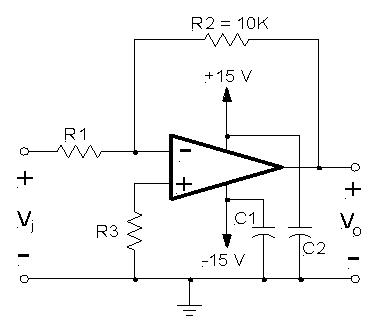
\includegraphics[]{img/ckt_tested}
  \caption{Circuit being tested.  $C_1 = C_2 = \SI{1}{\micro\farad}$}
  \label{fig:circuit}
\end{figure}

\subsection*{Test Configuration}
\label{sec:test_config}

\begin{figure}[hbtp]
  \centering
  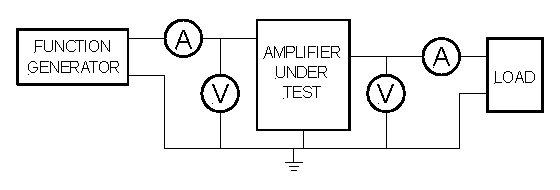
\includegraphics[]{img/test_config}
  \caption{Test Configuration}
  \label{fig:test_config}
\end{figure}

\section{Procedure}
\label{sec:procedure}

First, resistors $R_1$, $R_2$, and $R_3$ were measured with a
multimeter and recorded in Table~\ref{tab:table_01}.  Then the circuit
in Figure~\ref{fig:circuit} was constructed on a breadboard.  A function
generator was programmed to output a sine wave at \SI{1}{\kilo\hertz}.
The test configuration was constructed as shown in Figure 2 using
Fluke multimeters as the ammeters and an oscilloscope as both
voltmeters.  The function generator was added to the circuit as the
voltage input ($V_i$) and, with the oscilloscope measuring the voltage
generator, the amplitude was adjusted to $200\si{\volt_{rms}}$.  The
input voltage, input current, and output voltage were taken and
recorded in Table 2 with the open circuit across the load terminals.
Finally, the decade box was added to the output terminals (V0 in
Figure 1) of the circuit and, set to $200 \si{\ohm}$, and the output
voltage was measured and recorded in (Table 2).

\section{Results}
\label{sec:results}

\begin{table}[hbtp]
  \centering
  \begin{tabular}{*{4}{c}}
    \textbf{Name} & \textbf{Nominal} & \textbf{Measured} & \textbf{\% Error} \\
    & (\si{\kilo\ohm}) & (\si{\kilo\ohm}) & \\
    \hline
    $R_1$ & 1 & 0.986 & 1.40 \\
    $R_2$ & 10 & 9.88 & 1.20 \\
    $R_3$ & 1 & 0.983 & 1.70 \\
  \end{tabular}
  \caption{Comparison of labelled and actual resistance.}
  \label{tab:table_01}
  \end{table}

\begin{table}[hbtp]
  \centering
  \begin{tabular}{*{5}{c}}
    & \multicolumn{2}{c}{\textbf{Voltage}} & \multicolumn{2}{c}{\textbf{Current}} \\
    & $V_i$ & $V_o$ & $I_i$ & $I_o$ \\
    & (\si{\milli\volt_{rms}}) & (\si{\volt_{rms}}) & (\si{\milli\ampere_{rms}}) & (\si{\milli\ampere_{rms}}) \\
    \hline
    \textbf{No Load} & 200 & 1.98 & 0.2 & nil \\
    \textbf{Load} & 200 & 1.98 & 0.2 & 9.52 \\
  \end{tabular}
  \caption{Comparison of electrical characteristics of the amplifier under load.}
  \label{tab:table_02}
\end{table}

\begin{table}[hbtp]
  \centering
  \begin{tabular}{l*{5}{c}}
    & \multicolumn{3}{c}{\textbf{Load}} & \multicolumn{2}{c}{\textbf{No Load}} \\
    & \textbf{Nominal} & \textbf{Measured} & \textbf{\% Error} & \textbf{Nominal} & \textbf{Measured} \\
    \hline
    $R_o$ (\si{\ohm}) & 200 & 207.98 & 3.99\% & $\infty$ & $\infty$ \\
    $R_i$ (\si{\kilo\ohm}) & 1 & 1 & 0.00\% & 1 & 1 \\
    $A_v$ & 10 & 9.9 & 1.00\% & 10 & 9.9 \\
    $A_i$ & 50 & 47.6 & 4.80\% & nil & nil \\
    $G_m$ (\si{\siemens}) & 0.05 & 0.0495 & 1.00\% & 0 & 0 \\
    $R_m$ (\si{\kilo\ohm}) & 10 & 9.9 & 1.00\% & 10 & 9.90 \\
  \end{tabular}
  \caption{Comparison of values determined from amplifier models in Figure~\ref{fig:amp_models}}
  \label{tab:table_03}
\end{table}

\section{Conclusion}
\label{sec:conclusion}

As seen in Table 3, the measured results of the circuit were very
close to the calculated values using nominal values of the resistors.
This shows that the four amplifier models shown in
Figure~\ref{fig:amp_models} are closely representative of the
operational amplifier circuit seen in Figure 1.  The highest \%
difference when comparing the measured with the nominal theoretical
value was only 4.8\% (current gain [Ai] Table 3)!
\section{Appendix}
\label{sec:appendix}

\begin{figure}[h]
  \centering
  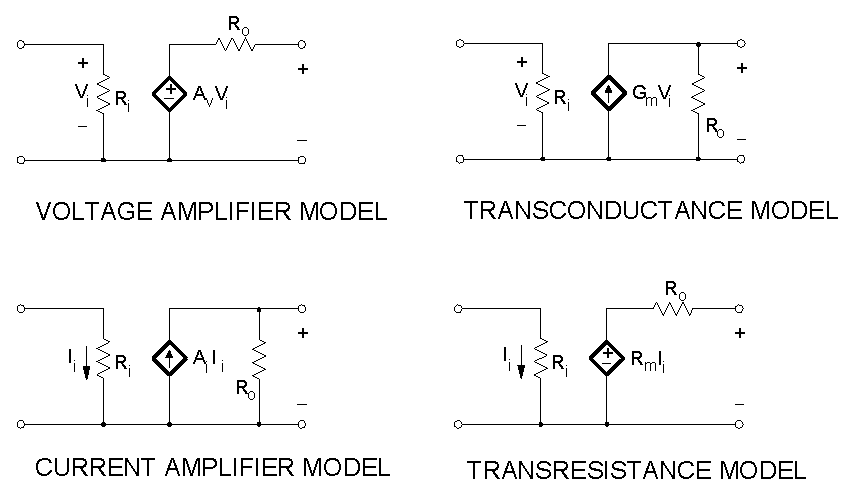
\includegraphics[width=\textwidth]{img/amp_models}
  \caption{Four equivalent models of an amplifier}
  \label{fig:amp_models}
\end{figure}

\subsection*{Equations}

% LaTeX sees blank lines as a start of another paragraph.  To avoid
% unnecessary vertical spaces between equations, and still visually
% separate in source, put a comment between them.
\begin{equation}
  \label{eqn:percent_error}
  \%_{error} = \frac{|measured - nominal|}{nominal} \times 100\%
\end{equation}
%
\begin{equation}
  \label{eqn:R_o}
  R_o = \frac{V_{noload} - V_{load}}{I_{load}}
\end{equation}
%
\begin{equation}
  \label{eqn:R_i}
  R_i = \frac{V_i}{I_i}
\end{equation}
%
\begin{equation}
  \label{eqn:A_v}
  A_v = \frac{V_o}{V_i}
\end{equation}
%
\begin{equation}
  \label{eqn:A_i}
  A_i = A_v \left(\frac{R_i}{R_o}\right)
\end{equation}
%
\begin{equation}
  \label{eqn:G_m}
  G_m = \frac{A_v}{R_o}
\end{equation}
%
\begin{equation}
  \label{eqn:R_m}
  R_m = A_v R_i
\end{equation}

\end{document}
